\documentclass[aspectratio=169,
hyperref={colorlinks,urlcolor=blue}
]{beamer}


%\usetheme{Pittsburgh}
\usetheme{default}
\usepackage{colortbl}%colored tables
%For using helvetica font:
\usepackage[scaled]{helvet}
\usepackage[T1]{fontenc}
\renewcommand\familydefault{\sfdefault}
\urlstyle{same} %sets the fonts for urls
\usepackage{pdfpages}
\usepackage{siunitx}
\usepackage{caption}
\usepackage{pifont}%for dings
\usepackage{pgfplots}%for 3d plotting
\pgfplotsset{compat = newest}
\usepackage{mathtools}%box in align env \Aboxed
\usepackage[american,smartlabels]{circuitikz}%for drawing circuits
\usepackage{multimedia}
\usepackage{animate}
\usepackage{xcolor}


\usetikzlibrary{arrows}
\usetikzlibrary {3d} 
\usetikzlibrary{decorations.markings, math}
\usetikzlibrary{intersections, pgfplots.fillbetween}
\usetikzlibrary {shapes.geometric} 


%\definecolor{myblue}{RGB}{5, 34, 150}
\definecolor{myblue2}{RGB}{5, 34, 150}
\definecolor{myblue}{RGB}{0,36,82}
\definecolor{myred}{RGB}{207, 2, 13}
\definecolor{mygreen}{RGB}{0, 158, 11}
\definecolor{myyellow}{RGB}{220,220,0}
\definecolor{qblue}{RGB}{0,36,82}
\definecolor{qgold}{RGB}{250,189,15}
\definecolor{qred}{RGB}{185,14,49}
\definecolor{cblue}{rgb}{0.13, 0.67, 0.8}
\definecolor{corange}{rgb}{0.8, 0.34, 0.0}
\definecolor{cpurple}{rgb}{0.54, 0.29, 0.42}

%%%%%%%%%%%% General settings
\setbeamercolor{frametitle}{fg=black}
\setbeamercolor{title}{fg=black}
\setbeamercolor{author}{fg=myblue2}

\beamertemplatenavigationsymbolsempty %no navigation controls at bottom of slides
%\setbeamertemplate{footline}[frame number]
\usefonttheme{professionalfonts} 
\setbeamerfont{title}{series=\bfseries,parent=structure}
\setbeamerfont{frametitle}{series=\bfseries,parent=structure}

%%%%%%%%%%%%Lists
\setbeamertemplate{itemize item}[circle] %{\color{myblue}$\circ$}
\setbeamertemplate{itemize subitem}{\color{myblue2}$\circ$}
\setbeamertemplate{itemize subsubitem}{\color{myblue2}$\cdot$}
\setbeamercolor{itemize item}{bg=myblue2,fg=myblue2}
\setbeamercolor{enumerate item}{bg=myblue2,fg=myblue2}
%%%%%%%%%%%%%%%%%%%%%%%%%%%%

%%%%%%%%%%%%Blocks
\setbeamertemplate{blocks}[rounded]
%Default block
\setbeamercolor{block title}{bg=myblue2, fg=white}
\setbeamercolor{block body}{bg=myblue2!10}
\setbeamerfont{block body}{size=\scriptsize}
\setbeamerfont{block title}{size=\scriptsize}
%Alert block
\setbeamercolor{block title alerted}{bg= myblue2, fg=white}
\setbeamercolor{block body alerted}{bg=myblue2!10}
\setbeamerfont{block body alerted}{size=\scriptsize}
\setbeamerfont{block title alerted}{size=\scriptsize}
%example block
\setbeamercolor{block title example}{bg=mygreen, fg=white}
\setbeamercolor{block body example}{bg=mygreen!10}
\setbeamerfont{block body example}{size=\scriptsize}
\setbeamerfont{block title example}{size=\scriptsize}
%%%%%%%%%%%%%%%%55


%%%%%%%%%%%%Figures and captions
\captionsetup{font=scriptsize,labelfont=scriptsize}
%\setbeamertemplate{caption}{\raggedright\insertcaption\par}
\newenvironment{capfig}[3]{\begin{figure}\includegraphics[width=#1\textwidth]{#2}\caption*{\textit{#3}}\end{figure}}{}

%\makeatother
%\setbeamertemplate{footline}
%{
%  \leavevmode%
%  \hbox{%
%  \begin{beamercolorbox}[wd=.4\paperwidth,ht=2.25ex,dp=1ex,center]{author in head/foot}%
%    \usebeamerfont{author in head/foot}\insertshortauthor
%  \end{beamercolorbox}%
%  \begin{beamercolorbox}[wd=.6\paperwidth,ht=2.25ex,dp=1ex,center]{title in head/foot}%
%    \usebeamerfont{title in head/foot}\insertshorttitle\hspace*{3em}
%    \insertframenumber{} / \inserttotalframenumber\hspace*{1ex}
%  \end{beamercolorbox}
%  }%
%  \vskip0pt%
%}
%\makeatletter

\makeatother
\setbeamertemplate{footline}
{
  \leavevmode%
  \hbox{%
\begin{beamercolorbox}[wd=.27\paperwidth,ht=2.25ex,dp=1ex,center]{author in head/foot}%
    \color{black}{\insertinstitute}
\end{beamercolorbox}
  \begin{beamercolorbox}[wd=.27\paperwidth,ht=2.25ex,dp=1ex,center]{author in head/foot}%
    \color{black}{\inserttitle}
  \end{beamercolorbox}%
  \begin{beamercolorbox}[wd=.27\paperwidth,ht=2.25ex,dp=1ex,center]{title in head/foot}%
    \color{black}{\insertshortauthor}
  \end{beamercolorbox}
  \begin{beamercolorbox}[wd=.27\paperwidth,ht=2.25ex,dp=1ex,center]{title in head/foot}%
    \hspace{.28\paperwidth}\color{black} \insertframenumber{} / \inserttotalframenumber\hspace*{1ex}
  \end{beamercolorbox}
  }%
  \vskip0pt%
}
\makeatletter

\setbeamertemplate{title page}
{
  \begin{tikzpicture}[remember picture,overlay]
    \def\barh{4}%15
  
    \draw[color=myblue2,line width=\barh] ([yshift=-0.5*\barh]current page.north west) -- ([yshift=-0.5*\barh,xshift=-0.67\paperwidth]current page.north east);
    \draw[color=myblue2,line width=\barh] ([yshift=-0.5*\barh,xshift=-0.67\paperwidth]current page.north east) -- ([yshift=-0.5*\barh,xshift=-0.34\paperwidth]current page.north east);
    \draw[color=myblue2,line width=\barh] ([yshift=-0.5*\barh,xshift=-0.34\paperwidth]current page.north east) -- ([yshift=-0.5*\barh]current page.north east); 
  
    \draw[color=myblue2,line width=\barh] ([yshift=0.5*\barh]current page.south west) -- ([yshift=0.5*\barh,xshift=-0.67\paperwidth]current page.south east);
    \draw[color=myblue2,line width=\barh] ([yshift=0.5*\barh,xshift=-0.67\paperwidth]current page.south east) -- ([yshift=0.5*\barh,xshift=-0.34\paperwidth]current page.south east);
    \draw[color=myblue2,line width=\barh] ([yshift=0.5*\barh,xshift=-0.34\paperwidth]current page.south east) -- ([yshift=0.5*\barh]current page.south east);
    %\node[left] at (current page.east) {
    %
\includegraphics[scale=0.1]{figures/coverpage}
    %};
  \end{tikzpicture}
  
  \usebeamerfont{title}\usebeamercolor[fg]{title}\inserttitle\par
  \usebeamerfont{subtitle}\usebeamercolor[fg]{subtitle}\insertsubtitle\par
  \vspace{2cm}
  \usebeamerfont{author}\usebeamercolor[fg]{author}\insertauthor\par
  \usebeamerfont{institute}\usebeamercolor[fg]{author}\insertinstitute\par
  \usebeamercolor[fg]{author}\par
  \usebeamercolor[fg]{titlegraphic}\inserttitlegraphic

} 

\setbeamertemplate{frametitle}{%
    \nointerlineskip%
        \par\hspace*{-\dimexpr0.5\paperwidth-0.5\textwidth}\textcolor{myblue2}{\rule{0.33\paperwidth}{6pt}}\textcolor{myblue2}{\rule{0.33\paperwidth}{6pt}}\textcolor{myblue2}{\rule{0.34\paperwidth}{6pt}} 
    \begin{beamercolorbox}[wd=\paperwidth,ht=0.75cm,dp=0.6ex]{frametitle}
        \hspace*{0.5cm}\strut\usebeamerfont{frametitle}\insertframetitle\strut
        %\hrule
    \end{beamercolorbox}%
    %%Line below:
%\par\hspace*{-\dimexpr0.5\paperwidth-0.5\textwidth}\textcolor{myblue}{\rule{\paperwidth}{0.4pt}}
     % <-- calculation of left margin width + rule
     %\textcolor{red}{\noindent\rule{\paperwidth}{2pt}}
}


%%%%%%%%%%%%Frame templates

%Slide with title
\newenvironment{titleframe}[1]
{\begin{frame}\frametitle{#1}\end{frame}}
{}

%Slide with title and itemize list:
\newenvironment{bulletframe}[1]
{\begin{frame}{#1} \itemize}
{\enditemize \end{frame}}

%Slide with two columns 50/50
\newenvironment{twocolframe}[3]
{\begin{frame}{#1}
 \begin{columns}[T]
 \column{0.5\textwidth}#2
 \column{0.5\textwidth}#3
 \end{columns}\end{frame}}{}

%Slide with two columns 60/40 <<<<<<<<<<<<<<<<<<<<<<  This one!
\newenvironment{twocolframesf}[3]
{\begin{frame}{#1}
 \begin{columns}[T]
 \column{0.6\textwidth}#2
 \column{0.4\textwidth}#3
 \end{columns}\end{frame}}{}
 
%Slide with two columns 70/30
\newenvironment{twocolframest}[3]
{\begin{frame}{#1}
 \begin{columns}[T] 
 \column{0.7\textwidth}#2
 \column{0.3\textwidth}#3
 \end{columns}\end{frame}}{} 
 
%Slide with two columns 40/60
\newenvironment{twocolframefs}[3]
{\begin{frame}{#1}
 \begin{columns}[T] 
 \column{0.4\textwidth}#2
 \column{0.6\textwidth}#3
 \end{columns}\end{frame}}{}
 
%Slide with two columns 70/30
\newenvironment{twocolframets}[3]
{\begin{frame}{#1}
 \begin{columns}[T] 
 \column{0.3\textwidth}#2
 \column{0.7\textwidth}#3
 \end{columns}\end{frame}}{} 

 
%Colloquium speaker (title, abstract, picture file, speaker name)
\newenvironment{colloquium}[5]
{
\begin{frame}{Colloquium: Friday 1:30pm in Stirling A}
\begin{columns}[T] 
 \column{0.8\textwidth}
 \textbf{#1}\\
 #2
 \column{0.2\textwidth}
 \capfig{#3}{#4}{#5}
 \end{columns}
\end{frame}
}
{} 

%%%%%%%%%%%%%Set Hyperref colors


\hypersetup{
  colorlinks=true,
  linkcolor=blue,    
  urlcolor=blue,     
  citecolor=blue      
}
%%%%%%%%%%%%%TOC bolding
\setbeamerfont{section in toc}{series=\bfseries}



%Frames:
% \twocolframesf 60/40 (fs, st, ts) 
% \titleframe
% bulletframe


%%%%%%%%%%%%%%%%%%%%%%%%%
%%%%%% START OF PRESENTATION %%%%%%
%%%%%%%%%%%%%%%%%%%%%%%%%

\title{Model and Experiment}
\institute{Theories, Uncertainty, and Dimensions}
\author{Building Models to Describe our World}


\begin{document}

%%%%%%%%%%%%%%%%%%%%%%%%%
%%%%%% Title slide %%%%%%
%%%%%%%%%%%%%%%%%%%%%%%%%
\begin{frame}
\titlepage
\thispagestyle{empty}

\begin{textblock*}{5cm}(11cm,4cm)
    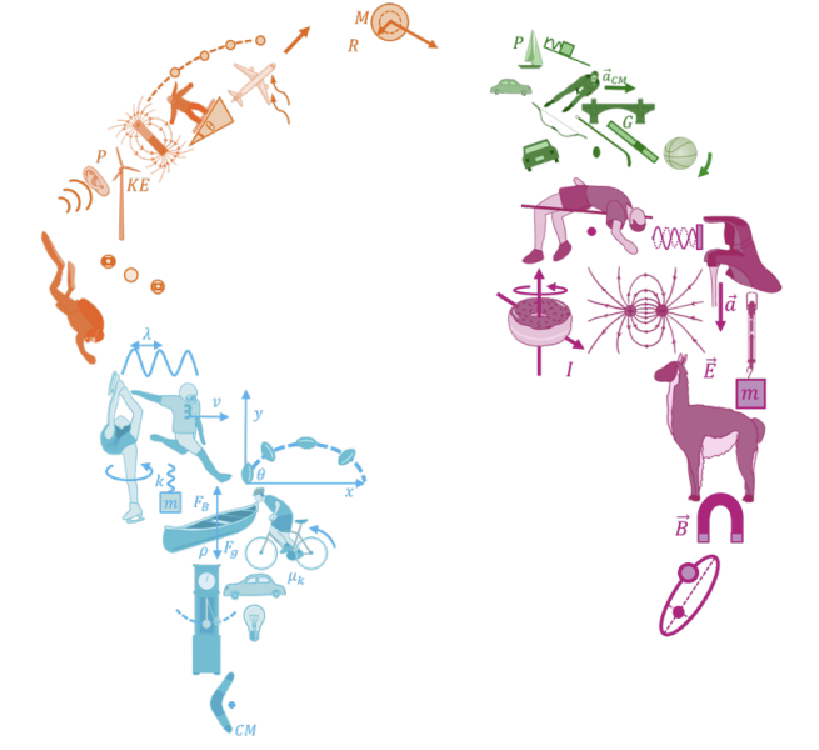
\includegraphics[width=4cm]{../figures/BMDW/logo}
\end{textblock*}

\end{frame}

%%%%%%%%%%%%%TOC

\twocolframe{Outline}
{\tableofcontents[sections=1-2, subsectionstyle=show/show]}
{\tableofcontents[sections=3, subsectionstyle=show/show]}

%%%%%%%%%%%%%%%%%%%%%%%%%











%%%%%%%%%%%%%%%%%%%%%%%%%%%%%%%%
\section{Building Models}
\label{sec:1dkinematics}
\title{Building Models}
\institute{Model and Experiment}
\author{\insertsubsection}


%%%%%%%%%%%%%%%%%%%%%%%%%
\begin{frame}
\titlepage
\thispagestyle{empty}
\end{frame}

%%%%%%%%%%%%%%%%%%%%%%%%%%%%






\subsection{Model vs experiment}
\label{subsec:modelvsexperiment}
\twocolframest{Model and experiment}
{
\begin{itemize}
\item We wish to test a theory, so we plan an experiment. That’s the fundamental aspect of science!
\item We use the theory to build a model and predict the result that we expect from our experiment
\item We compare the experimental result to the model prediction. Neither can ever be known with infinite precision:
\begin{itemize}
\item Model prediction depends on the assumptions that were made and uncertainties in the parameters of the model
\item Measurement depends on experimental uncertainties
\end{itemize}

\item[$\rightarrow$] Science can never make definitive statements, only statements based on probabilities (the probability that global warming is not due to human activity is very small, the probability that smoking does not cause lung cancer is very small…).
\end{itemize}
}
{  
\capfig{1}{../figures/ModelAndExperiment/doubt}{}
}


%%%%%%%%%%%%%%%%%%%%%%%%%%%%%%%%
\subsection{Does my prediction make sense?}
\label{subsec:doesmypredictionmakesense}
\begin{bulletframe}{Does my model prediction make sense?}
\item Did I correctly apply the rules for using a given theory? (e.g. identify all of the forces on an object, when applying Newton’s theory)
\item Does my predicted value have the correct order of magnitude? (e.g. did I predict that a ball will fall faster than the speed of light?)
\item Does my predicted value have the correct dimension? (e.g. did I predict that it would take a time of 3m to fall a distance of 1m?)
\item Does my predicted value change as I expect that it would? (e.g. if I drop a ball from higher, does my predicted fall time increase?)
\item[$\rightarrow$] \textbf{In assignments, we will require you to include a few sentences to evaluate whether your predictions make sense.}
\end{bulletframe}


%%%%%%%%%%%%%%%%%%%%%%%%%%%%%%%%
\subsection{Base dimenions and units}
\label{subsec:basedimensionsandunits}
\twocolframesf{Base dimensions and units}
{
\begin{itemize}
\item Anything that you can measure/quantify has a dimension.
\item Multiple units can be used for the same dimension (e.g mm, ft, soccer fields are all units for the dimension of length, L).
\item We can define a set of Base Dimension, and any other dimension can always be expressed in terms of those base dimensions. (e.g the dimension of speed is L/T)
\item Base SI units are the SI units that correspond to the base dimensions. (e.g. the SI unit for speed is m/s)
\end{itemize}
}
{
\scriptsize
\begin{center}
\begin{tabular}{ll }
\textbf{Dimension}&\textbf{SI unit}\\
\hline
\hline
Length [L]& meter [m]\\ \hline
Time [T]& seconds[s] \\ \hline
Mass [M]& kilogram [kg]\\ \hline
Temperature [$\Theta$]& kelvin [K] \\ \hline
Electric current [I]& amp\`ere [A]\\ \hline
Amount of substance [N]& mole [mol] \\ \hline
Luminous intensity [J]& candela [cd] \\ \hline
Dimensionless [1]& unitless [] \\ \hline
\end{tabular}
\captionof*{table}{\label{tab:modelandexperiment:SIunits}\textit{Base dimensions and their SI units with abbreviations.}}
\end{center}
You don’t need to memorize these, you will know them with practice (in general, don’t memorize things in physics, just ask if we forgot something on the formula sheet!)
}


%%%%%%%%%%%%%%%%%%%%%%%%%%%%%%%%


%%%%%%%%%%%%%%%%%%%%%%%%%%%%%%%%
\begin{frame}{Algebra with dimensions/units}
\begin{itemize}
\item If you obtain a formula for your model prediction, that prediction will have dimensions, based on the inputs to your model
\item For example, distance, $x$, in terms of an acceleration, $g$, initial speed, $v_0$, and time, $t$:
\begin{eqnarray}
x=v_0t+\frac{1}{2}gt^2
\end{eqnarray}
\item Evaluating the dimension of $x$:
\begin{eqnarray}
[x] = [v_0][t]+\left[\frac{1}{2}\right][g][t^2]=\frac{L}{T}T+1\frac{L}{T^2}T^2=L+L
\end{eqnarray}
\item You can use the SI units instead of the dimensions, to carry out the same exercise
\item \textbf{Always check that your prediction is dimensionally correct!} It won’t guarantee that your formula is correct, but it will identify if it is definitely wrong!
\end{itemize}

\end{frame}




%%%%%%%%%%%%%%%%%%%%%%%%%%%%%%%%









%%%%%%%%%%%%%%%%%%%%%%%%%%%%%%%%
\section{Uncertainty and Error}
\label{sec:uncertaintyanderror}
\title{Uncertainty and Error}
\institute{Model and Experiment}
\author{\insertsubsection}


%%%%%%%%%%%%%%%%%%%%%%%%%
\begin{frame}
\titlepage
\thispagestyle{empty}
\end{frame}

%%%%%%%%%%%%%%%%%%%%%%%%%%%%








%%%%%%%%%%%%%%%%%%%%%%%%%%
\subsection{Uncertainties}
\label{subsec:measurementuncertainty}
\begin{bulletframe}{Measurement uncertainty}
\item You can never measure anything to infinite precision.
\item You can only ever say that a value is likely within some range.
\item We communicate this as:
\begin{eqnarray}
x = (10.0\pm 0.1)\text{m}\;\;\; \rightarrow\;\;\;\text{``central value'' $\pm$ ``uncertainty''}
\end{eqnarray}
\item We mean that we are \emph{pretty confident} that $x$ is between \SI{9.9}{m} and \SI{10.1}{m}.
\item It is up to us, scientists, to \textbf{be precise} in explaining what we mean by \emph{pretty confident} $\rightarrow$ usually, we are 68\% confident. Ultimately, we need to be precise in describing how we determined the central value and uncertainty.
\end{bulletframe}


%%%%%%%%%%%%%%%%%%%%%%%%%%%%%%%%
\begin{bulletframe}{Relative uncertainty}
\item We want to know how precise our measurement is.
\item In other words, is the uncertainty large? Are we confident that the true value is close to the central value?
\item We quantify how large the uncertainty is relative to the central value $\rightarrow$ relative uncertainty:
\begin{align*}
x &=\bar x \pm \sigma_x\\
\text{Relative uncertainty} &=\frac {\sigma_x}{\bar x}=\frac{\text{uncertainty}}{\text{central value}}
\end{align*}
\item Express the relative uncertainty in percent
\item Usually, we consider 1\% relative uncertainty as precise
\item You measured that the Moon is $1\pm 1$ light years from the Earth; ok, good for you, but your very imprecise measurement is not very useful to test any model!
\end{bulletframe}

%%%%%%%%%%%%%%%%%%%%%%%%%%%%%%%%
\begin{bulletframe}{Determining an uncertainty}
\item This is by far the trickiest part of experimental physics, and usually the main focus of any experiment.
\item There is no “set in stone” rule for determining uncertainties, but there are some guidelines and accepted methods.
\item \textbf{The most important part is that you precisely describe (and justify) how you determined an uncertainty, and that you make every effort to minimize it.}
\item Ideally, if you can repeat a measurement multiple times; then this is the best way to determine an uncertainty:
\begin{itemize}
\item Mean and standard deviation (you’ll get practice in the labs next week)
\item Mean is the average, standard deviation is the average distance of measurements to the mean (whether or not the measurements are very scattered about the mean)
\end{itemize}
\item If appropriate, you can use half the smallest division of your measuring device as the uncertainty (it should rarely be smaller than this).
\end{bulletframe}

%%%%%%%%%%%%%%%%%%%%%%%%%%%%%%%%
\subsection{Precision vs accuracy  vs errors}
\label{subsec:}
\twocolframest{Precision and accuracy, random and systematic errors}
{
\begin{itemize}
\item You might find that multiple measurements have a small spread (and result in a small uncertainty) $\rightarrow$ Your measurements are \emph{precise}.
\item You later discover that your measurements are “way off” from the true value $\rightarrow$ Your measurements are not \emph{accurate}.
\item \textbf{Random error:} the spread in values that you get when repeating a measurement.
\item \textbf{Systematic error:} the offset of your measurement from the “true” value. In “real” science, this is very difficult to detect, since we never know the true value.
\item In first year physics, if you measure $g=5\pm 1$\si{m/s^2}, there is likely a systematic error
\end{itemize}
}
{
\capfig{1}{../figures/ModelAndExperiment/precision}{}
}

%%%%%%%%%%%%%%%%%%%%%%%%%%%%%%%%

%%%%%%%%%%%%%%%%%%%%%%%%%%%%%%%%
\twocolframesf{Human error}
{
\begin{itemize}
\item \textbf{That’s not a thing. Don’t use that term!}
\item Do you mean that you made a mistake? Then fix it!
\item Do you mean that, due to reaction time, you have a systematic uncertainty in your time measurement? Then include that error!
\item Do you mean that, due to parallax, you have a systematic uncertainty in your length measurement? Then include that error!
\end{itemize}
}
{
\capfig{1}{../figures/ModelAndExperiment/humanerror}{TAs grading lab reports}
}

%%%%%%%%%%%%%%%%%%%%%%%%%%%%%%%%


%%%%%%%%%%%%%%%%%%%%%%%%%%%%%%%%


%%%%%%%%%%%%%%%%%%%%%%%%%%%%%%%%
\subsection{Propogating uncertainties}
\label{subsec:propogatinguncertainties}
\twocolframesf{Propagating uncertainties}
{
\begin{itemize}
\item You measured, say, distance, $x$, and time, $t$, and want to know speed, $v$:
\begin{align*}
x&=\bar x \pm \sigma_x \\
t&=\bar t \pm \sigma_t \\
v&=v(x,t)=\frac{x}{t}=\bar v \pm \sigma_v 
\end{align*}
\item You want to propagate the uncertainties in $x$ and $t$ to determine the uncertainty in $v$
\item Derivative method + adding in quadrature:
\begin{align*}
\bar F &= F(\bar x, \bar y)\\
\sigma_F &= \sqrt{\left(\frac{\partial F}{\partial x} \sigma_x\right)^2+\left(\frac{\partial F}{\partial y} \sigma_y\right)^2}
\end{align*}
\end{itemize}
}
{
\begin{exampleblock}{When $F(x,y)\rightarrow v(x,t)$}
\begin{itemize}
\item<1-> Central value:
\begin{align*}
\bar v = \frac{\bar x}{\bar t}
\end{align*}
\item<2-> Uncertainty:
\begin{align*}
\only<2->{\sigma_v &= \sqrt{\left(\frac{\partial v}{\partial x} \sigma_x\right)^2+\left(\frac{\partial v}{\partial t} \sigma_t\right)^2}}\\
\only<3->{\frac{\partial v}{\partial x} &= \frac{\partial}{\partial x}\frac{x}{t}=\frac{1}{t}}\\
\only<4->{\frac{\partial v}{\partial t} &= \frac{\partial}{\partial t}\frac{x}{t}=\frac{-x}{t^2}}\\
\only<5->{\therefore \sigma_v &= \sqrt{\frac{1}{\bar t^2}\sigma_x^2+\frac{\bar x^2}{\bar t^4}\sigma_t^2}}
\end{align*}
\item<5> phew!
\end{itemize}
\end{exampleblock}
}

%%%%%%%%%%%%%%%%%%%%%%%%%%%%%%%%
\begin{frame}{Simple prescriptions}
\begin{itemize}
\item The derivative rule leads to simple prescriptions in most cases.
\item In practice, we’ll show you how to use a computer and QExpy to propagate uncertainties (see Appendix D).
\end{itemize}
\scriptsize
\begin{table}[H]
\centering
\begin{tabular}{p{2.5in}p{2in}} 
\textbf{Operation to get $z$} &\textbf{Uncertainty in $z$} \\
\hline
\hline
$z=x+y$ (addition) &  $\sigma_z=\sqrt{\sigma_x^2+\sigma_y^2}$ \\ \hline
$z=x-y$ (subtraction) & $\sigma_z=\sqrt{\sigma_x^2+\sigma_y^2}$ \\ \hline
$z=xy$ (multiplication) & $\sigma_z=xy\sqrt{\left(\frac{\sigma_x}{x}\right)^2+\left(\frac{\sigma_y}{y}\right)^2}$ \\ \hline
$z=\frac{x}{y}$ (division) & $\sigma_z=\frac{x}{y}\sqrt{\left(\frac{\sigma_x}{x}\right)^2+\left(\frac{\sigma_y}{y}\right)^2}$ \\ \hline
$z=f(x)$ (a function of 1 variable) &$\sigma_z=\left|\frac{df}{dx}\sigma_x \right|$ \\ \hline
\end{tabular}
\caption*{\label{tab:modelandexperiment:prop_uncertainties}\textit{How to propagate uncertainties from measured values $x\pm\sigma_x$ and $y\pm\sigma_y$ to a quantity $z(x,y)$ for common operations. Addition and subtraction: use absolute uncertainties. Multiplication and division, use relative uncertainties}.}
\end{table}
\end{frame}

%%%%%%%%%%%%%%%%%%%%%%%%%%%%%%%%


%%%%%%%%%%%%%%%%%%%%%%%%%%%%%%%%






%%%%%%%%%%%%%%%%%%%%%%%%%%%%%%%%
\section{Dimensional Analysis}
\label{sec:dimensionalanalysis}
\title{Dimensional Analysis}
\institute{Model and Experiment}
\author{\insertsubsection}


%%%%%%%%%%%%%%%%%%%%%%%%%
\begin{frame}
\titlepage
\thispagestyle{empty}
\end{frame}

%%%%%%%%%%%%%%%%%%%%%%%%%%%%






%%%%%%%%%%%%%%%%%%%%%%%%%%%%%%%

\twocolframesf{Dimensional analysis}
{
\begin{itemize}
\item Sometimes, you know that a certain quantity, $z$, must depend on other quantities, $x$ and $y$, but you have no idea how to model it:
\begin{eqnarray*}
z=f(x,y)=x^ay^b
\end{eqnarray*}
\item As a minimum, you know that you must combine $x$ and $y$ in a way that the combination has the dimensions of $z$, but you want to know the powers, $a$ and $b$. 
\item Suppose that:
\begin{eqnarray*}
[z]=\frac{L}{T^2},\quad [x]=M\quad [y]=\frac{ML}{T^2}
\end{eqnarray*}
\end{itemize}
}
{
\begin{exampleblock}{Determining $a$ and $b$}
\begin{itemize}
\item<1-> $[z] = [x]^a[y]^b$
\item<2-> $\frac{L}{T^2}=(M)^a\left(\frac{ML}{T^2} \right)^b=(M)^{a+b}\frac{L^{b}}{T^{2b}}$
\item<3->[$\rightarrow$] Equate powers of $L$, $T$ and $M$ on both sides:
\item<4-> On the left, $M$ is to the power of 0 (there are no $M$s) and $M$ is to the power $a+b$ on the right. These must be the same:\\
$0=a+b$
\item<5-> Same with $L$ (1 on the left, $b$ on the right):\\
$1=b$
\item<6->[$\rightarrow$] $b=1$ and $a=-1$. $f(x,y)=x^ay^b$ must thus be of the form:
\begin{eqnarray*}
z = x^{-1}y^{1}=\frac{y}{x}
\end{eqnarray*}
\end{itemize}

\end{exampleblock}
}

%%%%%%%%%%%%%%%%%%%%%%%%%%%%%%%%



%%%%%%%%%%%%%%%%%%%%%%%%%%%%%%%%



%%%%%%%%%%%%%%%%%%%%%%%%%%%%%%%%






\end{document}



